\documentclass[12pt, letterpaper]{article}
\usepackage{graphicx}
\usepackage[T1]{fontenc}
\usepackage[polish]{babel}
\usepackage[utf8]{inputenc}

\graphicspath{{images/}}

%--------------------------------------------------------------------------------------------------
%       TITLE SECTION
%--------------------------------------------------------------------------------------------------
\begin{titlepage}
 

\includegraphics[scale=0.2]{ur_inf_logo}\\ \\ \\ \\

\begin{center}
	{ \huge \bfseries Programowanie obiektowe}\\[0.4cm] 

	\textsc{\Large Aplikacja bankowa}\\[0.5cm] \\ \\ \\ \\ 
	
	\vspace{0.8cm}	
	
	\emph{Autorzy:} \\
	\textbf{Oskar Paśko} (117987)\\
	\textbf{Eliza Tworkowska} (119003)	
	
	
	\vspace{0.8cm}
	
	\emph{Kierunek:} \\
	Informatyka i ekonometria
	
	\vspace{8cm}
	
	\emph{Prowadzący:} \\
	mgr inż. Ewa Żesławska\\ \\ \\ \\ 
	
	\vspace{2cm}
	
	Rzeszów, 2023
\end{center}
\end{titlepage}
%--------------------------------------------------------------------------------------------------
%      END TITLE SECTION
%--------------------------------------------------------------------------------------------------

\begin{document}
\newpage

%--------------------------------------------------------------------------------------------------
%      SPIS TREŚCI
%--------------------------------------------------------------------------------------------------
\tableofcontents

\newpage

%--------------------------------------------------------------------------------------------------
%      OPIS ZAŁOŻEŃ
%--------------------------------------------------------------------------------------------------
\section{Opis założeń projektu}

\quad Niniejszy projekt dotyczy aplikacji bankowej, która ma za zadanie ułatwić klientowi
z korzystania z dostępnych na rynku usług bankowych.

\quad Użytkownik posiadający konto w bazie danych niniejszej aplikacji może się zalogować do niej za pomocą swojego numeru klienta oraz hasła. Na głównej stronie może sprawdzić swoje aktualne saldo, na które składają sie salda wszystkich jego kart posiadanych w banku. Tabela ze wszystkimi kartami widoczna jest w centralnym punkcie strony głównej. Dodatkowo, na stronie głównej, użytkownik może sprawdzić historię transakcji. Ponadto klient może dokonać wpłaty na wybraną przez siebie kartę oraz wypłaty z wybranej przez siebie karty z założeniem, że posiada na niej wystarczającą ilość środków. Dzięki aplikacji możliwe jest również dokonanie przelewów z założeniami takimi 
jak w przypadku wpłat i wypłat. Użytkownik ponadto może dodać nową kartę płatniczą lub usunąć isniejącą przy 
założeniu,że jej bilans wynosi 0 zł.

\newpage

%--------------------------------------------------------------------------------------------------
%      SPECYFIKACJA WYMAGAŃ
%--------------------------------------------------------------------------------------------------
\section{Specyfikacja wymagań}

\subsection{Wymagania funkcjonalne}
\begin{itemize}
\item Aplikacja oferuje połączenie z bazą danych.
\item Bank oferuje usługi użytkownikom zarejestrowanym w aplikacji.
\item Bank oferuje możliwość zarejestrowania się nowym użytkownikom.
\item Klient może wpłacić lub wypłacić pieniądze z wybranej karty.
\item Klient może dokonać przelewu na wybraną kartę.
\item Klient może sprawdzić saldo swoich kart płatniczych.
\item Klient może sprawdzić historię przelewów.
\item Zarejestrowany klient może dodać nową kartę płatniczą do swojego konta.
\end{itemize}

\newpage

\subsection{Wymagania niefunkcjonalne}
\begin{itemize}
\item Możliwość dodawania, usuwania oraz edycji rekordów w bazie podczas działania aplikacji.
\item Aplikacja jest przyjazna dla klienta i jego rodziny oraz jest prosta\\ w użyciu.
\item Aplikacja tworzona jest w języku Java.
\item Aplikacja nawiązuje połączenie z bazą danych w języku MySQL i używa rekordów w niej zapisanych.
\end{itemize}

\newpage

%--------------------------------------------------------------------------------------------------
%      OPIS TECHNICZNY BAZY DANYCH
%--------------------------------------------------------------------------------------------------
\section{Opis techniczny bazy danych}

\subsection{Opis założeń}

\quad Baza danych przechowuje dane klientów oraz należących do nich kart płatniczych, jak również  
historię wykonanych przelewów.\\

\quad Podczas działania aplikacji na bazie danych zostają wykonywane działania wyświetlania, modyfikowania, wstawiania oraz usuwania danych.

\subsection{Diagram ERD}

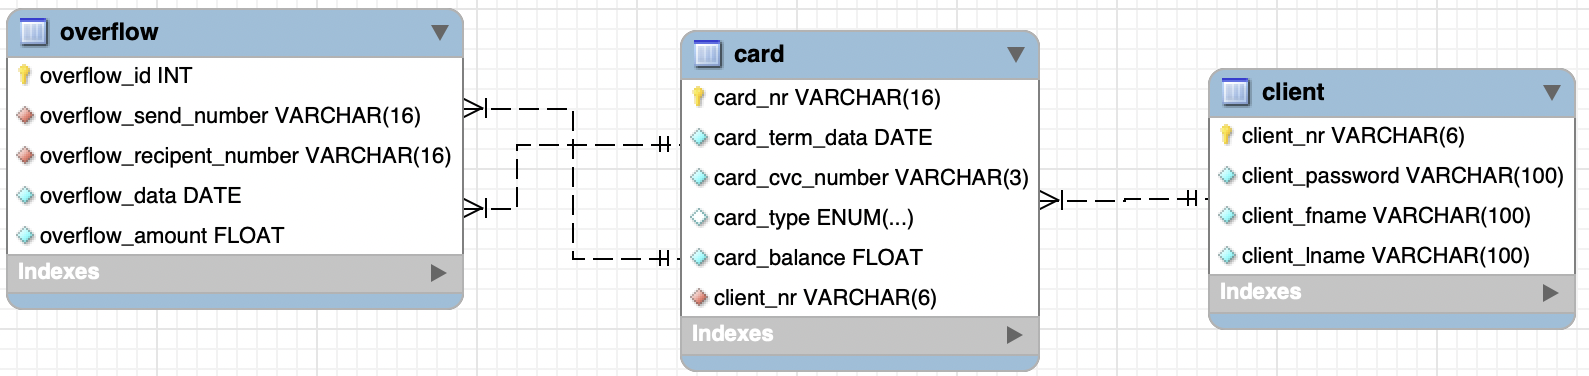
\includegraphics[scale=0.5]{erd}

\subsection{Opis tabel w bazie danych}

\subsubsection{Tabela client}

\quad Tabela "client" przechowuje informacje na temat klienta. Przechowywane informacje to sześciocyfrowy numer klienta, który jest kluczem głównym tabeli, hasło klienta oraz imię i nazwisko klienta.\\


\subsubsection{Tabela card}

\quad Tabela "card" przechowuje informacje o kartach płatniczych klientów.\\ W tabeli przechowujemy informacje o szesnastocyfrowym numerze karty, który pełni rolę klucza głównego, datę ważności karty, numer zabezpieczający cvc, który jest zawsze trzycyfrowy, typ karty, saldo znajdujące się na karcie oraz numer klienta posiadającego daną kartę. Numer ten jest zapisany jako klucz obcy tabeli połączony metodą wiele do jednego z tabelą "client".



\subsubsection{Tabela overflow}

\quad Tabela "card"  przechowuje informacje o przelewach dokonanych przez klienta. W tabeli przechowujemy klucz główny tabeli, numer karty, z której został wysłany przelew oraz numer karty, 
na którą został wysłany przelew. Dodatkowo przechowuje datę wykonania przelewu oraz jego wartość.

%--------------------------------------------------------------------------------------------------
%      SYSTEM KONTORLI WERSJI
%--------------------------------------------------------------------------------------------------

\section{System kontroli wersji}

\quad Projekt realizowany był z wykorzystaniem systemu kontroli wersji Git,\\ a wszystkie pliki źródłowe projektu znajdują się pod adresem:\\  \url{https://www.github.com/oskarpasko/BankApp} . 

%--------------------------------------------------------------------------------------------------
%      OPIS TECHNICZNY PROJEKTU
%--------------------------------------------------------------------------------------------------
\section{Opis techniczny projektu}
\begin{itemize}
\item Języki programowania: Java, MySQL
\item Środowiska programistyczne: IntelliJ IDEA, MySQL Workbench
\item Wersja SDK: 18.0.2
\item Aplikacja tworzona na komputery z systemem Windows oraz macOS
\end{itemize}

\section{Tabela}

\begin{center}
\begin{tabular}{|c|c|c|}
\hline
cell1 & cell2 & cell3 \\
cell4 & cell5 & cell6 \\
cell7 & cell8 & cell9 \\
\hline
\end{tabular}
\end{center}


\end{document}